
\documentclass[11pt]{article}
\usepackage[paper=letterpaper, margin=.5in]{geometry}
\pdfpagewidth 8.5in
\pdfpageheight 11in
\setlength\parindent{0in}

%% AMS PACKAGES - Chances are you will want some or all of these if writing a math dissertation.
\usepackage{amsmath, amscd, amssymb, amsthm, multirow, enumerate, multicol, graphicx, listings}
\newcommand{\Z}{\mathbb{Z}}
\newcommand{\R}{\mathbb{R}}
\newcommand{\Q}{\mathbb{Q}}
\newcommand{\C}{\mathbb{C}}
\newcommand{\N}{\mathbb{N}}
\newcommand{\V}{\mathbb{V}}
\newcommand{\U}{\mathcal{U}}
\newcommand{\del}{\partial}
\newcommand{\real}{\textrm{Re }}
\newcommand{\imag}{\textrm{Im }}
\newcommand{\pd}[2]{\frac{\partial #1}{\partial #2}}
\newcommand{\deriv}[2]{\frac{d #1}{d #2}}
\newcommand{\sumk}{\sum_{k=1}^\infty}
\newcommand{\sumj}{\sum_{j=1}^\infty}
\newcommand{\sumn}{\sum_{n=0}^\infty}
\newcommand{\summ}[2]{\sum_{k=#1}^{#2}}
\newcommand{\sig}[1]{\sum_{#1 =1}^\infty}
\newcommand{\un}[1]{\bigcup_{#1 =1}^\infty}
\newcommand{\inter}[1]{\bigcap_{#1 =1}^\infty}
\newcommand{\ip}[2]{\langle #1, #2 \rangle}
\newcommand{\ipxu}{\langle x,u_j \rangle}
\newcommand{\uj}{\{u_j\}_{j=1}^\infty}
\newcommand{\B}{\mathcal{B}}

\newcommand{\E}{\mathrm{E}}
\newcommand{\var}{\mathrm{Var}}
\newcommand{\cov}{\mathrm{Cov}}
\newcommand{\ST}{mbox{ s.t. }}

\newcommand{\Example}{\noindent {\bf Example. \quad} }
\newcommand{\Proof}{\noindent {\bf Proof: \quad} }
\newcommand{\Remark}{\noindent {\bf Remark. \quad} }
\newcommand{\Remarks}{\noindent {\bf Remarks. \quad} }
\newcommand{\Case}{\noindent {\underline{Case} \quad} }

\newcommand{\st}{ \; \big | \:}

\newcommand{\deuc}{d_{\mathrm euc}}
\newcommand{\dtaxi}{d_{\mathrm taxi}}
\newcommand{\ddisc}{d_{\mathrm disc}}
\newtheorem{theorem}{Theorem}[section]
\newtheorem{lemma}[theorem]{Lemma}
\newtheorem{proposition}[theorem]{Proposition}
\newtheorem{corollary}[theorem]{Corollary}
\theoremstyle{definition}
\newtheorem{definition}[theorem]{Definition}
\newtheorem{example}[theorem]{Example}

\begin{document}
%%%%%%%%%%%%%%%%%%%%%%%%%%%%%%%%%%%%%%%%%%%%%%%%%%%%%%%%%%%%%%%%%%%%%%%%%%%%%%%%%%%%%%%%%%%%%%%%%%%%%%%%%%%%%%%%%%%%%%%%%%%%%%%%%%%%%
Homework 4 \hfill Aaron Maurer
\vspace{2mm}
\hrule
\vspace{2mm}
\begin{itemize}
    \item[1.]
        \begin{itemize}
            \item[a)]
                \begin{align*}
                    \|Q\beta - y\|^2 &= (Q\beta - y)^T(Q\beta - y) \\                
                                     &= (\beta^T Q^T - y^T)(Q\beta - y) \\
                                     &= \beta^TQ^TQ\beta - y^TQ\beta - \beta^T Q^T y + y^Ty  \\
                                     &= (\beta^T\beta - y^TQ\beta - \beta^T Q^T y + y^TQQ^Ty) + (y^Ty - y^TQQ^Ty) \\
                                     &= (\beta^T - y^TQ)(\beta + Q^Ty) + (y^Ty - y^TQQ^Ty- y^TQQ^Ty + y^TQQ^Ty) \\
                                     &= \|\beta - Q^Ty\|^2 + (y^Ty - y^TQQ^Ty- y^TQQ^Ty + y^TQQ^TQQ^Ty) \\
                                     &= \|\beta - Q^Ty\|^2 + (y^T - y^TQQ^T)(y - QQ^Ty)\\
                                     &= \|\beta - Q^Ty\|^2 + \|y - QQ^Ty\|^2\\
                \end{align*}
            \item[b)]
                Since $Q^T$ is orthogonal,
                \[RSS(\beta) = \|Y-X\beta\|^2 = \|Q^TY-Q^TX\beta\|^2 = \|Q^TY - RP^T\beta\|^2 \]
                Using the result from a, we have that
                \[RSS(\beta) = \|QRP^T\beta - Y\|^2 = \|RP^T\beta-Q^TY\|^2 + \|Y-QQ^TY\|^2 \]
                Since \(\|y-QQ^Ty\|^2\) is fixed, the $RSS$ will be at a minimum when \(\|RP^T\beta-Q^TY\|^2\) is minimized. If \(R=\mathbf{0}\), then trivially all \(\beta\) achieve the same $RSS$. Otherwise, we want to minimize the non-trivial part of the expression. Where $R_{11}$ has $m$ rows, let $Q_1$ be the first $m$ rows of $Q$ with $Q_2$ the remainder. Thus, 
                \begin{align*}
                \|RP^T\beta-Q^TY\|^2 &= \left\| \left[\begin{array}{cc} R_{11} & R_{12} \\ \mathbf{0} & \mathbf{0} \end{array} \right] P^T \beta - [Q_1^T Q_2^T]Y \right \|^2 \\
                    &= \| \left[R_{11} R_{12}\right] P^T \beta - Q_1^T Y \|^2 + \|Q_2^T Y\|^2
                \end{align*}
                Since $\|Q_2^TY_2\|^2$ is also fixed, we can reduce our minimization problem to minimizing 
                \[\| [R_{11} R_{12}] P^T \beta - Q_1^T Y \|^2\]
                Thus, we will get a minimum when,
                \[ \left[R_{11} R_{12}\right] P^T \beta = Q_1^T Y \]
            \item[c)]
                We want to solve the expression above. Let \(W=\left[R_{11} R_{12}\right] P^T\). If we have some solution $\beta$, and a vector $a$ in the null space of \(W\), then 
                \[ W(\beta+a) = W \beta + W a = Q_1^T Y + 0 \]
                So $\beta+a$ is also a solution. Let $\beta^*$ be the vector that achieves the smallest norm and solves the equation. Assuming $R$ isn't all $0$, then there is some $\beta$ perpendicular to all $a$. If $\beta_1$ is and another $\beta_2$ isn't, by Cauchy-Schwartz
                \begin{align*}
                    \|\beta_2+a\|^2 &\geq \|\beta_1 + a\|^2 \\
                    \|\beta_2\|^2 + \|a\|^2 &> \|\beta_1\|^2 + \|a\|^2 \\
                    \|\beta_2\|^2 &> \|\beta_1\|^2 \\
                \end{align*}
                Thus, $\beta^*$ must be perpendicular to all $a$. If $b$ is a vector, 
                \[0= b^T W a = (W^Tb)^T a \]
                So the range of \(W^T\) is perpendicular to all $a$ as well. Thus, since $\beta^*$ is perpendicular to the null space of \(W\), it must be in the range of \(W^T\) (This range fills the complement of the null space because taking the transpose of a matrix doesn't reduce its rank). Accordingly, for some $v$,
                \begin{align*}
                    \beta^* &= W^Tv \\
                    W\beta^* &= WW^Tv \\
                    Q_1^T Y &= WW^Tv  \\
                    W^T(WW^T)^{-1} Q_1^T Y &= W^T v \\
                    W^T(WW^T)^{-1} Q_1^T Y &= \beta^*  \\
                \end{align*}
                Thus we have our answer. We can invert \(WW^T\) since \(W\) is full row rank (since \(R_{11}\) is invertible) and similarly \(W^T\) is full column rank.
            \item[d)]
                Here is the implemented R script:
                \lstinputlisting[firstline=8,lastline=19]{hw4.R}
            \item[e)]
                The two sets of coefficients are identical, except for the coefficients for pop75. In the normal regression, the coefficient was -1.6915, while in the solution to the singular version, the coefficients are both -.8457. \(-.8457+-.8457=-1.6915\) because the total additive effect needs to be the same. For any $a$, \(-1.6915a\) and \(-1.6915(1-a)\) would have accomplished this, but since we insisted on the smallest norm, we got $a=.5$, which is the minimum of \((-1.6915a)^2+(-1.6915(1-a))^2\).
            \item[f)]
                It seems like a robust heuristic to compute the rank of $R$ would be to count the number of entries on the diagonal which have a magnitude above a very small threshold (maybe $1e^{-10}$. Here, the diagonal for the second occurrence of pop75 is $-1.7e^{-15}$, despite the fact that variable is linearly dependent on the first occurrence of pop75 and should be $0$. Thus, it seems like the $QR$ has small rounding errors which we could exclude by this heuristic. \\
                If $R$ is not singular but extremely close, this suggests that a robust approach would be to exclude the variables which have an extremely small diagonal value in $R$, or, alternatively, treat them as singular and use the method developed in this problem to find $\beta$.
        \end{itemize}
        
    \item[2.]
        \begin{itemize}
            \item[a)]
                We know that when $A=BC$, $a_{ij}=b_i c_j$, where $b_i$ and $c_j$ are respectively the $i$th row and $j$th column of $B$ and $C$. Further, if $C$ is itself the product of matrices $D$ and $E$, then $c_j=De_j$, where $e_j$ is the $j$th column of $D$. Combining this, $a_{ij}=b_i D e_j$. If we treat the $i$th and $j$th rows of $X$ as column vectors on their own, this leads to the conclusion that
                \[h_{ij}=x_i^T(X^TX)^{-1}x_j\]
                \smallskip
                Since $H$ is symmetric and idempotent,
                \[h_{ii}=\sum_{j=1}^n h_{ij}h_{ji} = \sum_{j=1}^n h_{ij}^2 \]
                Also, if \(J=\{j:x_i=x_j\}\), then for all \(j\in J\),
                \[h_{ij} = x_j^T (X^TX)^{-1} x_i = x_i^T (X^TX)^{-1} x_i = h_{ii} \]
                So, combining these,
                \begin{align*}
                    h_{ii} &= \sum_{j=1}^n h_{ij}^2 \\
                    h_{ii} &= r h_{ii}^2 + \sum_{j\not\in J} h_{ij}^2 \\
                    h_{ii} &\geq r h_{ii}^2 \\
                    \frac{h_{ii}}{r} &\geq h_{ii}^2  \\
                    \frac{1}{r} &\geq h_{ii} \\
                \end{align*}
                \smallskip
                If $X$ includes a column of $1$s at the front (for an intercept), then $\mathbf{1}_n$ is in the span of $H$ and $H\mathbf{1}_n=\mathbf{1}_n$. We may conclude that 
                \[\sum_{j=1}^n h_{ij} = 1 \]
                This would imply that, since $\sum_{j=1}^n h_{ij}^2$ is minimized when $h_{ij}=\frac{1}{n}$ for all $h_{ij}$,
                \[\sum_{j=1}^n h_{ij}^2 \geq \sum_{j=1}^n \frac{1}{n^2} = \frac{1}{n} \]
                Combining this with what we showed earlier,
                \[h_{ii} = \sum_{j=1}^n h_{ij}^2 \geq \frac{1}{n}\]
                Giving us the desired results that 
                \[\frac{1}{r} \geq h_{ii} \geq \frac{1}{n} \]
            \item[b)]
                When $X$ is an invertible matrix, 
                \[\sum_{i=1}^n h_{ii} = \mathrm{tr}(H) = \mathrm{rk}(H) = n\]
                So $h_{ii}=1=\frac{1}{r}$, since $r=1$ for all $i$. If $X$ is just one row repeated $n$ times, then $\mathrm{rk}(X)=1$, and 
                \[\sum_{i=1}^n h_{ii} = \mathrm{tr}(H) = \mathrm{rk}(H) = 1 \]
                So it must be the case that $h_{ii}=1=\frac{1}{n}$
        \end{itemize}
    \item[3.]
        \begin{itemize}
            \item[a)]
                Under the normal assumption,
                \[ \hat\beta \sim N_p(\beta,\sigma^2(X^TX)^{-1}) \]
                So we can also assume 
                \[ R\hat\beta \sim N_q(R\beta,\sigma^2R(X^TX)^{-1}R^T) \]
                In turn since, $z$ is independent of $Y$, and thus independent of $\hat\beta$, 
                \begin{align*}
                     z &\sim N_q(R\beta, \sigma^2 \mathbb{I}_q) \\
                    \Rightarrow  R\hat\beta - z &\sim N_q(R\beta - R\beta,\sigma^2R(X^TX)^{-1}R^T+\sigma^2 \mathbb{I}_q) \\
                    \Rightarrow  \frac{R\hat\beta - z}{\sigma} &\sim N_q(\mathbf{0},(R(X^TX)^{-1}R^T+\mathbb{I}_q))
                \end{align*}
                Accordingly, we would expect that 
                \[\frac{\frac{1}{q}(R\hat\beta - z)^T(R(X^TX)^{-1}R^T+\mathbb{I}_q)^{-1}(R\hat\beta - z)}{\hat\sigma^2} \sim F_{q,n-p} \]
                So we would get a confidence set of 
                \[ E_\alpha = \left\{\beta\in \R^q : (R\hat\beta - z)^T(R(X^TX)^{-1}R^T+\mathbb{I}_q)^{-1}(R\hat\beta - z) \leq q\hat\sigma^2 f_{q,n-p,\alpha} \right\} \]
            \item[b)]
                I have plotted the confidence intervals for where $z$ will land:
                \begin{center}
                    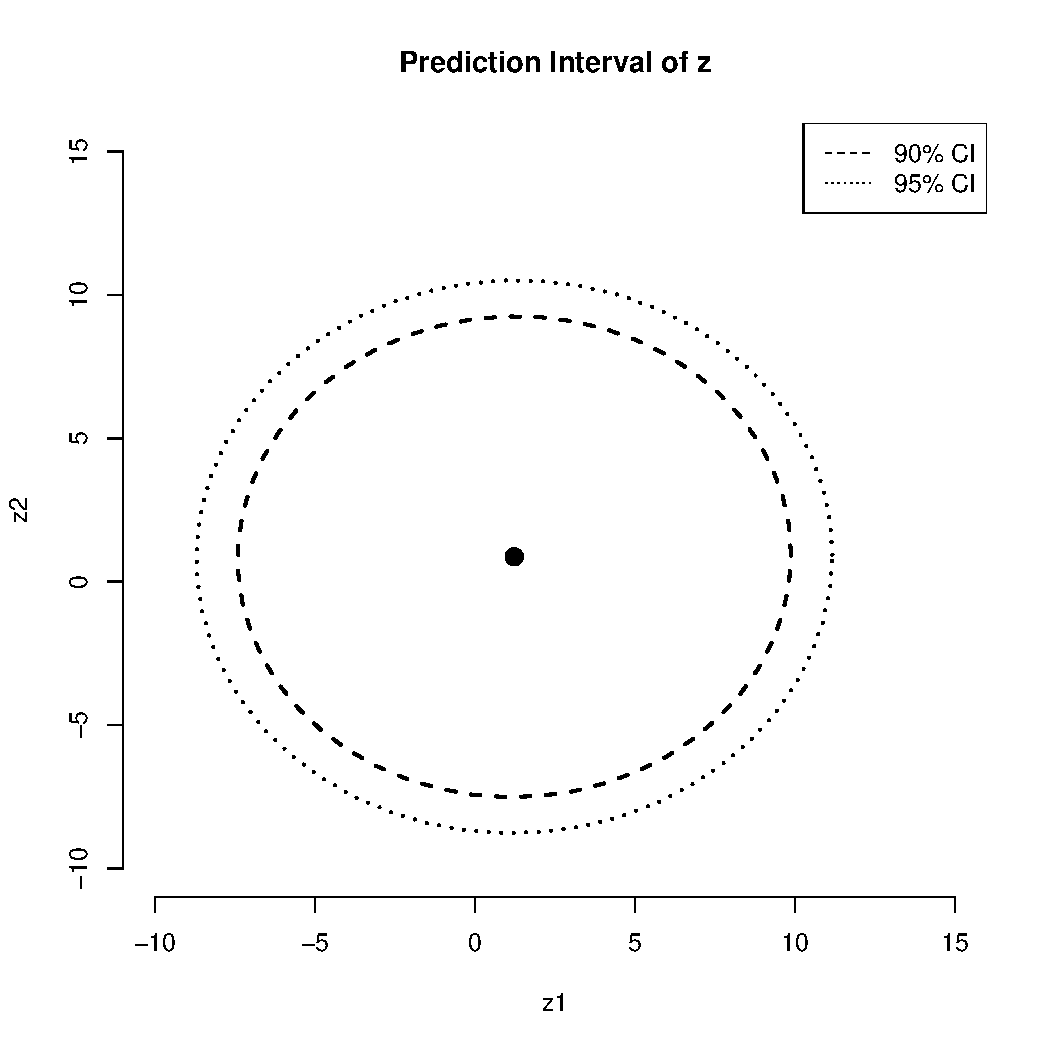
\includegraphics[width=12cm]{hw4_3_b_ci} 
                \end{center}
                You will notice that the confidence interval is very close to a circle. If we create just a confidence interval for \(R\hat\beta\), it is a very elongated ellipse, with the main axis not parallel to the $z1$ or $z2$ axis. However, the noise of $z$ around$R\beta$ has no covariance, and there is equal variance in the direction of $z1$ and $z2$, so if it we created a confidence interval for it conditioned on a $R\beta$, we would get a circle. Since the magnitude variance of $z$ around $X\beta$ is much higher than the variance of the estimate of $R\hat\beta$, this makes the confidence interval close to a circle.
                Here is the R code I used:
                \lstinputlisting[firstline=38,lastline=65]{hw4.R}
            \item[c)]
                Having repeated the simulation $1000$ times, $z$ fell within the $90\%$ confidence interval $91.3\%$ of the time, which indicates that my expression for the confidence interval was pretty accurate. I calculated whether or not the simulated data point fell in the confidence interval using exactly the formulation from part a. I've attached the code:

                \lstinputlisting[firstline=68,lastline=79]{hw4.R}
            
                
        \end{itemize}
    \item[4.]
        \begin{itemize}
            \item[2.13.]
                \begin{itemize}
                    \item[1.]
                        Looking over this plot, simple linear regression looks extremely plausible for this model. We see what looks like a linear relationship between the two variables with a multivariate normal noise distribution, which is exactly what we would want.
                        \begin{center}
                            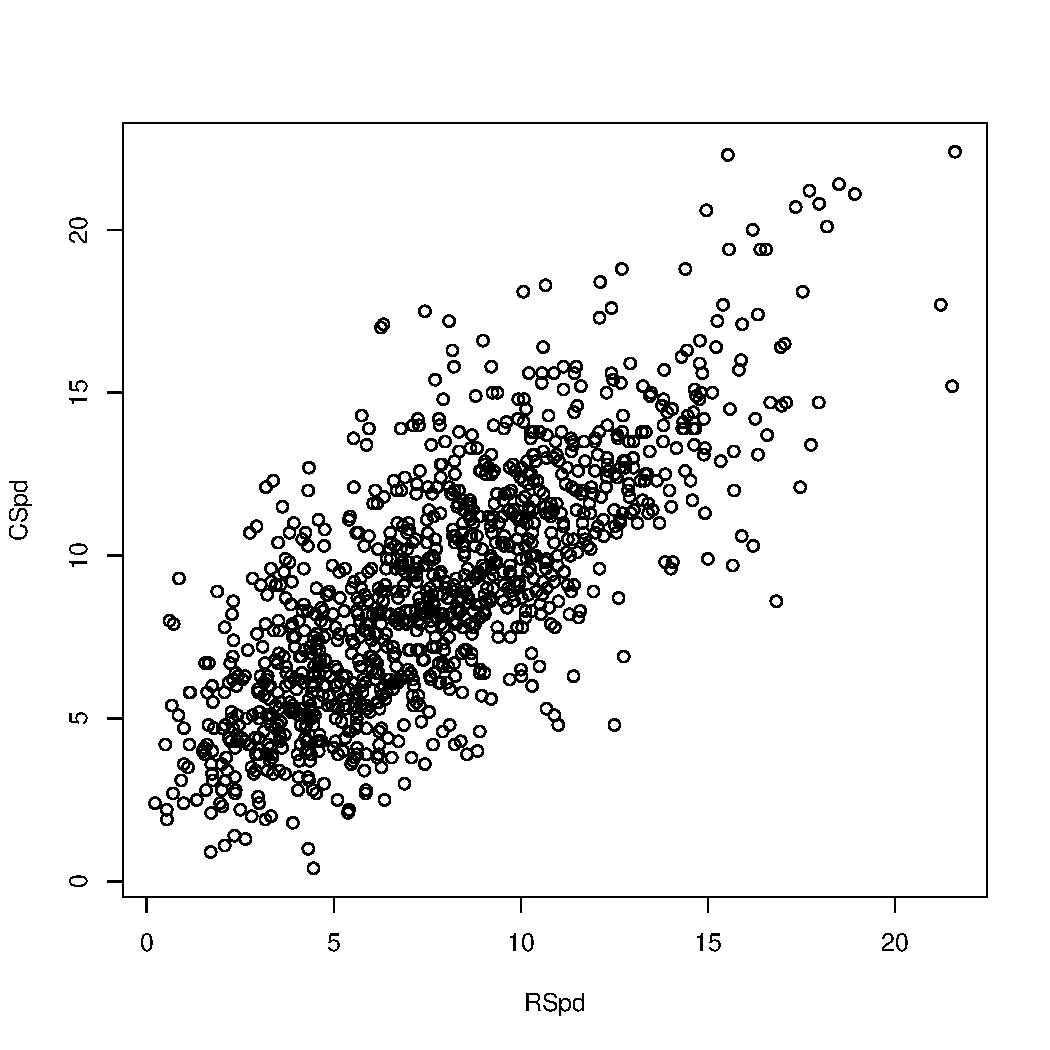
\includegraphics[width=12cm]{hw4_4_2_13_1_plot} 
                        \end{center}
                    \item[2.]
                        For the coefficients, we get \\
                        \begin{tabular}{c | c c c c}
                            & Estimate & Std. Error & t value & Prob \\
                            \hline
                            Intercept & 3.141 & .120 & 18.52 & $<$2e-16 \\
                            RSpd      & .756 & .020 & 38.50 & $<$2e-16
                        \end{tabular} \\
                        These coefficients are both quite meaningful, the t values indicating that there is a negligible probability of the estimates being positive by chance if each coefficient was actually 0. The most interesting is the coefficient on RSpd, which indicates that their is a strong correlation between the wind speed at the two sites. Additionally, we have a residual standard error on $2.466$ degrees of freedom, an R-squared of $.5709$, and a F-statistic of $1482$ on $1$ and $1114$ degrees of freedom, resulting in a p-value of $<2e-16$. This speaks very strongly that this regression is meaningful; it explains $57\%$ of the original variance, and the probability that we would see these results if we just had a mean model is negligible.
                    \item[3.]
                        From the model, we get a prediction that when the wind at the reference site was $7.4285$, we would see wind at the test site of $\hat y_0 = [1 \> 7.4285]\beta = 8.7552$. We predict with $95\%$ certainty, based on the normality assumption, that the actual test site wind speed would be in the range \(\hat y_0 \pm t_{1114}^{.025} \hat\sigma\sqrt{1 + [1\> 7.4285]^T(X^TX)[1\> 7.4285]} = (3.914,13.570) \).
                    \item[4.]
                        Starting with the mean of the prediction, 
                        \begin{align*}
                            \frac{1}{m} \sum_{i=1}^m \hat y_{*i} x &= \frac{1}{m} \sum_{i=1}^m (x_{*i}\beta_1 + \beta_0) \\ 
                            \frac{1}{m} \sum_{i=1}^m \hat y_{*i} x &= \hat\beta_0 + \frac{1}{m} \sum_{i=1}^m (x_{*i}\beta_1) \\ 
                            \frac{1}{m} \sum_{i=1}^m \hat y_{*i} x &= \hat\beta_0 + \frac{\hat\beta_1}{m} \sum_{i=1}^m (x_{*i})  \\ 
                            \frac{1}{m} \sum_{i=1}^m \hat y_{*i} x &= \hat\beta_0 + \hat\beta_1 \bar x  
                        \end{align*}
                        So we conclude the prediction for the mean is equal to the mean of the predictions. If we call the prediction at $\bar x_*$ $\bar y_*$ and the expectation $\hat y_*$, then
                        \begin{align*}
                            \var(\bar y_*) &= \var(\bar y_* - \hat y_* + \hat y_m ) \\  
                            \var(\bar y_*) &= \var(\bar y_* - \hat y_*) + \var(\hat y_*) -2\cov(\bar y_* - \hat y_*,\hat y_*) \\  
                            \var(\bar y_*) &= \frac{\hat\sigma^2}{m} + \hat\sigma^2\left(\frac{1}{n} + \frac{(\bar x_* - \bar x)^2}{SXX} \right) \\  
                            se \>\bar y_* &= \sqrt{\frac{\hat\sigma^2}{m} + \hat\sigma^2\left(\frac{1}{n} + \frac{(\bar x_* - \bar x)^2}{SXX} \right)}   
                        \end{align*}
                        We know the covariance term is equal to $0$ since the residuals and the predictions are orthogonal, and thus have $0$ covariance.
                    \item[5.]
                        We can plug the values given and from the data set into the above equation to get the standard error. We get a $\sigma^2=6.082$ from the regression, $\bar x=7.778$, and $SXX= 15785.56$ from the data. Thus, the standard error is:
                        \[ se \>\bar y_* = \sqrt{\frac{6.082}{62039} + 6.082\left(\frac{1}{1116} + \frac{(7.429 - 7.778)^2}{15785.56} \right)} = .075 \]   
                        Combining this with the model's prediction of the expectation of $\bar y_*=8.7552$ from earlier, we get a $95\%$ confidence interval of 
                        \[\bar y_* \pm se(\bar y_*) t_{1114}^{.025} = (8.609,8.901) \]
                \end{itemize}

            \item[4.6.]
                When I bootstrapped the mean wind speed at the candidate site, I got a $95\%$ of the means landing in $(8.800,9.22)$. This is surprising, because its in general higher, and only partially overlaps with the analytic predicted confidence interval. So, I checked the assumption of normality:
                \begin{center}
                    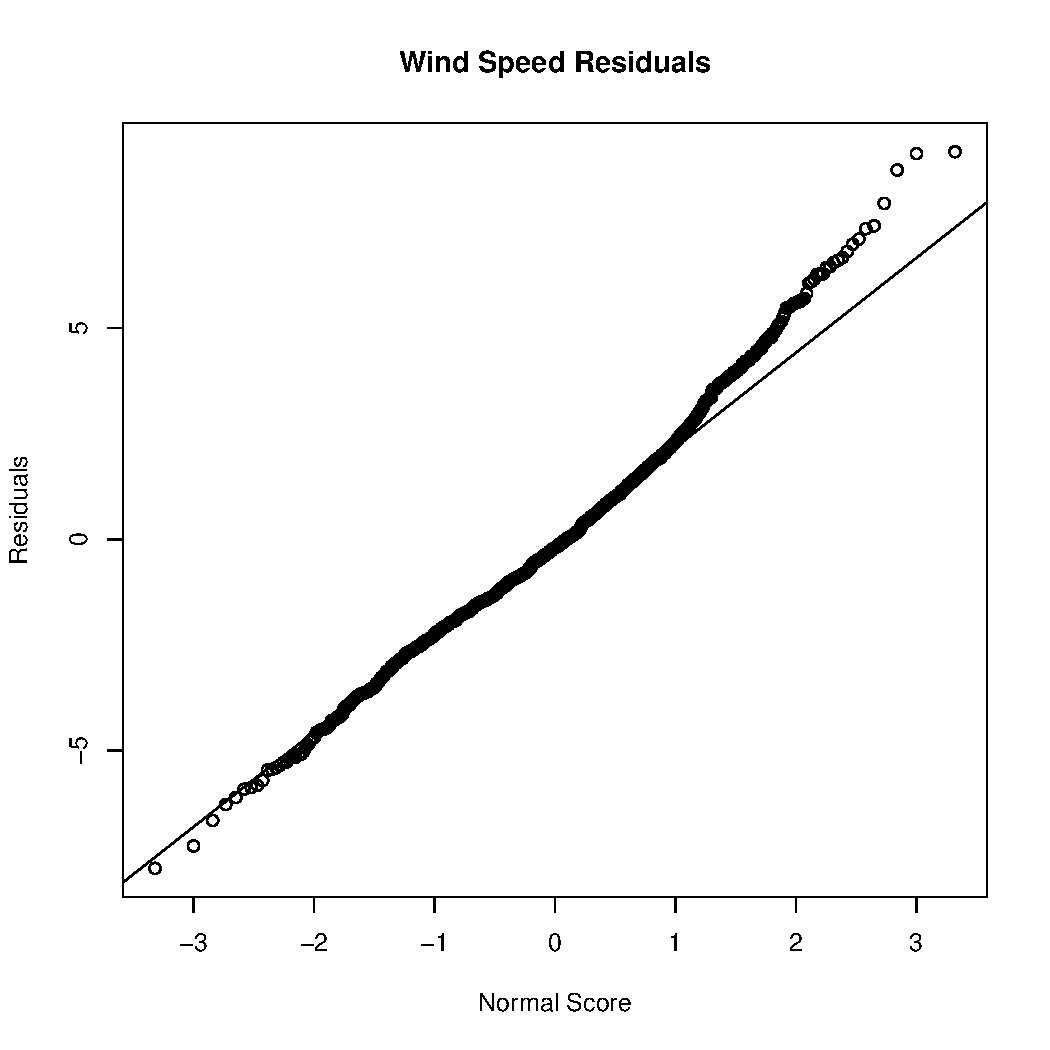
\includegraphics[width=12cm]{hw4_4_4pt6_qq} 
                \end{center}
                Here, the qq plot shows that the distribution of the residuals has a thicker tail than the normal distribution. This supports the notion that there is more variability than we assumed, and in particular the upper bound of the analytic confidence interval is too low, supporting the bootstrapped confidence interval.
        \end{itemize}


\end{itemize}



\end{document}
